%%%%%%%%%%%%%%%%%%%%%%%%%%%%%%%%%%%%%%%%%%%%%%%%%%%%%%%%%%%%%%%%%%%
% Chapter1: Introduction 
%%%%%%%%%%%%%%%%%%%%%%%%%%%%%%%%%%%%%%%%%%%%%%%%%%%%%%%%%%%%%%%%%%%

\chapter{Introduction}
\label{chap:intro}

\section{Background}

% viết từ time-series forecasting và các phương pháp tiếp cận (sơ bộ)
% Cùng với numerical, categorical, and text data, time-series data đang ngày càng trở nên phổ biến không chỉ ở nguồn sinh dữ liệu (e.g., lĩnh vực tài chính, năng lượng, vận tải,\dots) mà còn ở các phương pháp để phân tích và dự đoán chúng (e.g., phân rã tần số, các phương pháp dựa trên ghi nhớ dữ liệu quá khứ,\dots). Điều này là dễ hiểu vì phân tích và dự đoán time-series data mang lại những lợi ích lớn trong việc tổ chức, hoạch định chiến lược sản xuất và kinh doanh.

Time-series data is gaining popularity alongside numerical, categorical, and text data not only in terms of data sources (like finance, energy, and transportation), but also in terms of methods for analyzing and forecasting them (like frequency decomposition and methods based on historical data memorization). This makes sense as planning, organizing, and developing business strategies are greatly aided by the analysis and prediction of time-series data.

% Hai hướng tiếp cận chính được sử dụng trong phân tích và dự đoán time-series data là fundamental analysis và technical analysis \cite{ayitey2023forex}. Trong khi fundamental analysis thiên về phân tích các yếu tố tác động từ bên ngoài, vốn rất khó có thể capture từ các biến thiên giá trị trong quá khứ, như chính sách, chiến lược kinh tế của công ty, quốc gia để dự đoán tương lai; technical analysis dựa hoàn toàn vào lịch sử biến động giá trị để phân tích xu hướng tương lai.

The two main approaches used in analyzing and predicting time-series data are fundamental analysis and technical analysis \cite{ayitey2023forex}. While fundamental analysis concentrates on examining external factors that are hard to capture from past price changes, such as the economic strategies and policies of nations and businesses, technical analysis relies entirely on historical price changes to forecast future trends

% Chính vì tính phi cấu trúc trong các thông tin của tin tức, đạt được sự tự động hóa hiệu quả trong các phương pháp fundamental analysis là rất khó. Do đó, các nhà nghiên cứu thường tập trung phát triển các phương pháp technical analysis. Cùng với sự phát triển của machine learning và deep learning, các phương pháp trải dài từ Auto-regressive model (năm 1951) \cite{moran1951hypothesis}, Moving average model (năm 2000) \cite{rosenblatt2000gaussian}, đến Long Short-term memory model - \verb|LSTM| (năm 1997) \cite{hochreiter1997long} và Transformers \cite{vaswani2017attention} (năm 2017), được phát triển nhằm tự động hóa một cách thông minh quá trình dự báo.

It is challenging to achieve efficient automation of basic analytical methods due to the unstructured nature of news data. As a result, academics frequently concentrate on creating techniques for technical analysis. The forecasting process can now be intelligently automated with the help of machine learning and deep learning techniques, such as Auto-regressive model (1951) \cite{moran1951hypothesis}, Moving average model (2000) \cite{rosenblatt2000gaussian}, Long short-term memory model - \verb|LSTM| (1997) \cite{hochreiter1997long}, and Transformers (2017) \cite{vaswani2017attention}.

% thu hẹp lại aperiodic time-series data (phân tích 3 thách thức chính)
% Các phương pháp nêu trên và các biến thể chủ yếu hoạt động trên periodic time-series data (e.g., thời tiết, giao thông,...). Loại dữ liệu này thể hiện rõ tính chu kỳ, hoặc tính mùa vụ theo thời gian. Do đó, việc phân tích và dự đoán được diễn ra rất dễ dàng với độ chính xác cao. Điều này càng đúng hơn với các phương pháp hướng đến phân rã chu kỳ bằng các deep neural network hiện nay \cite{liu2022scinet,chen2021autoformer,zhou2022fedformer}. Tuy nhiên, rất ít nghiên cứu chú trọng đến \textbf{aperiodic time-series data} (e.g., foreign exchange rate, stock price,...).

The aforementioned techniques, together with their variations, are mostly applicable to periodic time-series data, such as traffic, weather, etc. Over time, this kind of data clearly shows a seasonal or cyclical character. As a result, analysis and prediction may be done quickly and accurately. This is especially true for existing techniques that use deep neural networks to try to decompose periods \cite{liu2022scinet,chen2021autoformer,zhou2022fedformer}. Nevertheless, \textbf{aperiodic time-series data} (e.g., stock prices, foreign exchange rates, etc.) has been the subject of very few investigations.

% Điểm khác biệt rất dễ nhận thấy ở aperiodic time-series data so với periodic time-series data nằm ở chỗ chúng không thể hiện một chu kỳ rõ ràng (see figure \ref{fig:ill_aperiodic}). Thật vậy, trong hình \ref{fig:periodic}, thuộc tính \textit{Temperature oil} (target variable) của tập dữ liệu Electricity Transformer Temperature (\verb|ETT-m2|) \cite{zhou2021informer} thể hiện tính chu kỳ rất rõ ràng theo thời gian vì nhu cầu sử dụng điện biến thiên theo mùa. Trong khi đó, \textit{Close price} between US dollar and Japanese yen (figure \ref{fig:aperiodic}) bị chi phối bởi rất nhiều yếu tố. Một tin tức mới về tình hình kinh tế cũng có thể gây ra tác động lớn lên tỷ giá này. Do đó, tỷ giá này không thể hiện bất kỳ tính chu kỳ nào.

As can be seen in figure \ref{fig:ill_aperiodic}, the primary distinction between aperiodic and periodic time-series data is their lack of a distinct periodicity. In fact, because of seasonal fluctuations in electricity demand, the \textit{Temperature oil} (target variable) attribute of the Electricity Transformer Temperature dataset (\verb|ETT-m2|) \cite{zhou2021informer} shows a very noticeable periodicity over time in figure \ref{fig:periodic}. In the meanwhile, a number of external factors influence the \textit{Close price} between the US dollar and the Japanese yen (figure \ref{fig:aperiodic}). This exchange rate can be significantly impacted by recent economic news. As a result, there is no periodicity in this exchange rate.

\begin{figure}[H]
    \centering
    \begin{subfigure}[b]{0.5\textwidth}
        \centering
        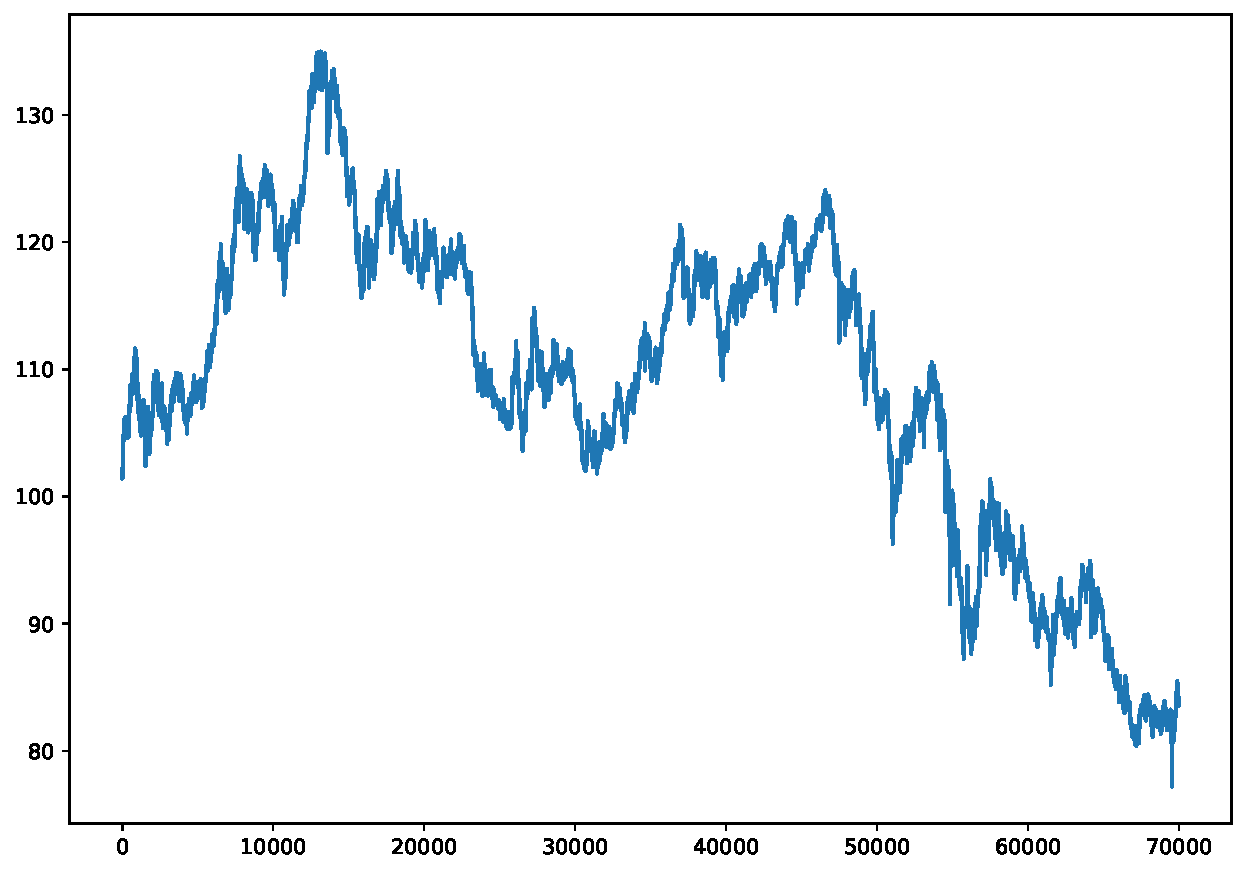
\includegraphics[width=\textwidth]{usd_close.pdf}
        \caption{Exchange ratio between USD and JPY.}
        \label{fig:aperiodic}
    \end{subfigure}%
    ~
    \begin{subfigure}[b]{0.5\textwidth}
        \centering
        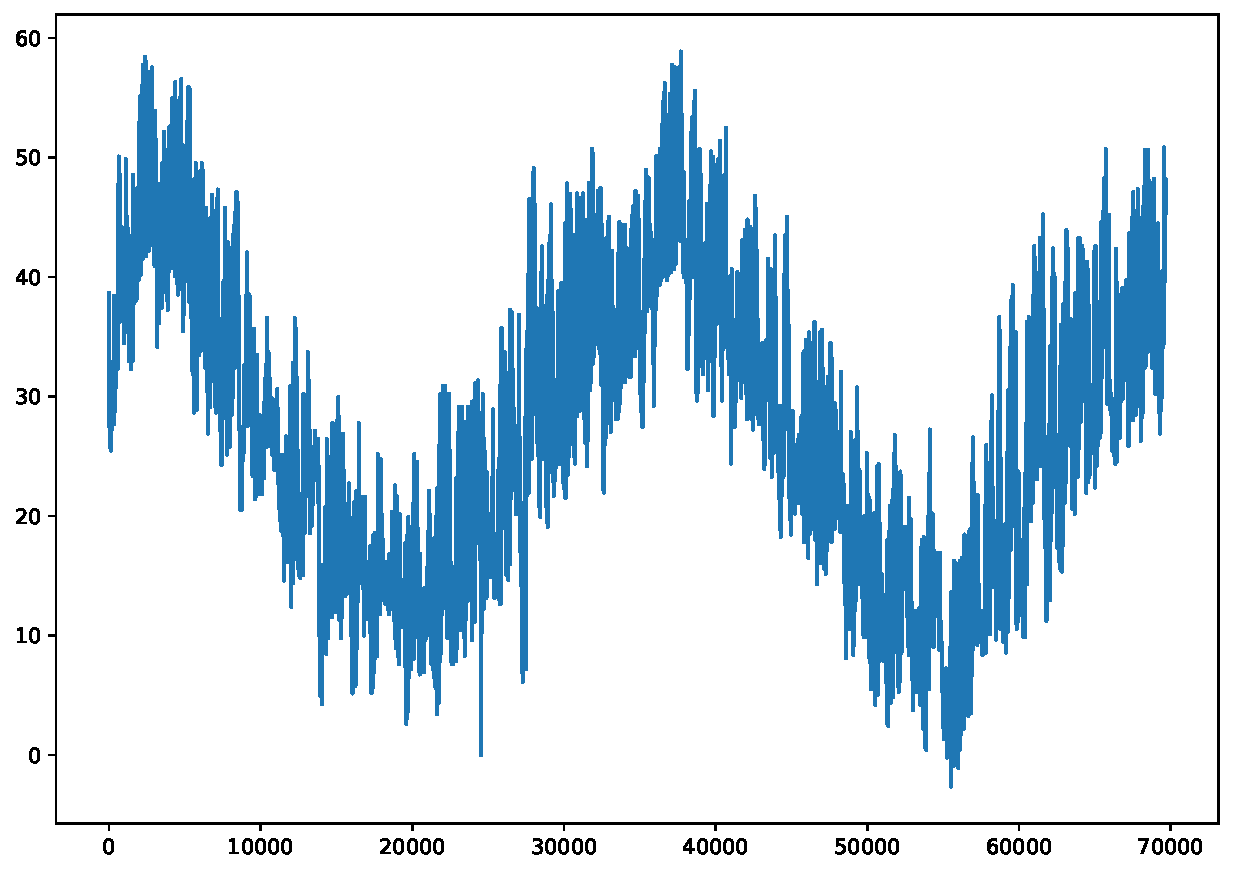
\includegraphics[width=\textwidth]{ett_OT.pdf}
        \cprotect\caption{\textit{Oil temperature} in \verb|ETT-m2| dataset.}
        \label{fig:periodic}
    \end{subfigure}

    \caption{70.000 samples of aperiodic (\ref{fig:aperiodic}) and periodic (\ref{fig:periodic}) time-series dataset.}
    \label{fig:ill_aperiodic}
\end{figure}

% Đặc điểm chính của aperiodic time-series data nằm ở chỗ dữ liệu này bị chi phối rất nhiều bởi các yếu tố bên ngoài như chiến lược sản xuất, chính sách kinh tế, chính trị của các công ty hay quốc gia. Chính điều này đã gây ra sự thay đổi đáng kể trong tính chất dữ liệu, hay còn biết đến là concept drift scenarios \cite{liu2025onsitnet}. Về mặt toán học, điều này khiến cho phương sai của aperiodic time-series data biến thiên liên tục với khoảng biến thiên rất rộng. Cũng chính điều này đã khiến cho việc rút trích đặc trưng trên dữ liệu thông qua một cửa sổ trượt gặp rất nhiều khó khăn do dữ liệu đã không còn thể hiện tính chu kỳ.

Aperiodic time-series data's primary feature is that it is heavily impacted by external factors, including production strategy and the political and economic policies of nations or businesses. This has resulted in notable modifications to the data's characteristics, which are also referred to as concept drift scenarios \cite{liu2025onsitnet}. Mathematically, this results in aperiodic time-series data with a continuous and incredibly wide variance. Additionally, because the data no longer exhibits periodicity, it becomes extremely challenging to extract characteristics from it using a sliding window.

% Tóm lại, làm việc trên aperiodic time-series data đối mặt với ba thách thức chính: (1) Dữ liệu bị ảnh hưởng rất nhiều bởi các yếu tố kinh tế, chính trị, xã hội; (2) Dữ liệu có phương sai lớn và không cố định; (3) Khó rút trích đặc trưng vì dữ liệu thể hiện tính phi chu kỳ rất mạnh. \textbf{Trong nghiên cứu này, chúng tôi tập trung giải quyết ba thách thức vừa nêu trong bài toán dự đoán xu hướng (tăng hoặc giảm) trên aperiodic time-series data.}

In conclusion, there are three primary obstacles to overcome when dealing with aperiodic time-series data: (1) External influences including politics, economy, and society have a significant impact on the data; (2) Data has a massive and non-stationary variance; and (3) Data's strong non-periodicity makes feature extraction challenging. \textbf{In this study, we focus on solving the three challenges mentioned above in the problem of trend prediction (upward or downward) on aperiodic time-series data.}

\section{Motivation}
\label{sec:moti}
% cần paraphrase lại

% viết về việc 3 thách thức chính được giải quyết nhưng chưa hiệu quả
% Trong ba thách thức nêu trên, thách thức đầu tiên là thách thức khó giải quyết nhất dựa trên các phương pháp technical analysis vì các thông tin về chính trị, xã hội rất khó để rút trích thông qua dữ liệu lịch sử của một tập dữ liệu. Tuy nhiên, theo efficient market hypothesis \cite{fama1970efficient}, chính các thông số trong dữ liệu lịch sử lại phản ánh rất rõ các thông tin về sự biến động của thị trường. Điều này nghĩa là, \textbf{bằng việc xem xét kỹ lưỡng lịch sử giao dịch, người ta hoàn toàn có thể nắm bắt được các biến động thị trường và dự báo được tương lai} mà không cần sử dụng đến các thông tin về chính trị, xã hội. Các nghiên cứu \cite{overreactioncontrarian, mech1993portfolio} cũng chỉ ra sự phụ thuộc giữa chỉ số tài chính của một công ty nhất định và chỉ số của các công ty khác. Nói cách khác, \textbf{việc tích hợp phân tích nhiều nguồn thông tin khác nhau thuộc cùng một lĩnh vực có thể mang lại những thông tin phân tích đáng giá cho các chỉ số đang quan tâm.}

In three aforementioned challenges, the first challenge is the most difficult to solve based on technical analysis methods because political and social information is difficult to extract through historical data of a data set. However, according to the efficient market hypothesis \cite{fama1970efficient}, historical data itself clearly reflects information about market fluctuations. That means, \textbf{by carefully examining the transaction history, one can completely grasp market fluctuations and forecast the future} without using political and social information. In addition, \cite{overreactioncontrarian, mech1993portfolio} studies also point out the dependence between the financial indicators of a certain company and the indicators of other companies. In other words, \textbf{integrating analysis of multiple sources of information within the same domain can yield valuable analytical insights for the indicator of interest.}

% Khi đối mặt với thách thức thứ hai, các mô hình ensemble thường được sử dụng để hạn chế ảnh hưởng của sự biến đổi variance \cite{ali2020complete, zafeiriou2020intraday, sadeghi2021combined}. Về cơ bản, các mô hình ensemble hoạt động dựa trên việc chia nhỏ dữ liệu thành nhiều phần và giả định một mức phương sai cố định trên các thành phần này sau đó mô phỏng lại sự biến thiên đó. Hướng tiếp cận này là hoàn toàn hợp lý vì một mô hình khó có thể nắm bắt được toàn bộ sự biến thiên của dữ liệu xuyên suốt một khoảng thời gian dài. \textbf{Bằng việc phân tích và tổng hợp thông tin từ nhiều sub-model, ensemble learning cung cấp một cái nhìn đa chiều về dữ liệu, giúp mô hình tổng quát thích ứng tốt với sự thay đổi mạnh mẽ của phương sai.}

When faced with the second challenge, ensemble learning is often used to mitigate the effects of variance \cite{ali2020complete, zafeiriou2020intraday, sadeghi2021combined}. Basically, ensemble learning works by splitting the data into multiple parts and assuming a fixed level of variance across these parts, then simulating that variation. This approach is reasonable because it is difficult for a single model to capture all the variability in the data over a long period of time. \textbf{By analyzing and synthesizing information from multiple sub-models, ensemble learning provides a multidimensional view of the data, which helps the overall model adapt well to strong variance changes.}

% Cho đến nay, rất nhiều mô hình được đề xuất để có thể rút trích đặc trưng trên dữ liệu nói chung và time-series data nói riêng. Điển hình trong số đó, Convolutional neural network - \verb|CNN| \cite{lecun1989handwritten}, \verb|LSTM| \cite{hochreiter1997long}, và cơ chế attention \cite{bahdanau2014neural, luong2015effective, vaswani2017attention} lần lượt được đề xuất để rút trích các đặc trưng cục bộ, ghi nhớ các đặc trưng ngắn-dài hạn, và nhấn mạnh các vector trong ma trận đặc trưng. \textbf{Bằng việc sử dụng hiệu quả các phương pháp này, các ràng buộc ẩn trong aperiodic time-series data có thể được rút trích một cách hiệu quả}, giúp vượt qua thách thức thứ ba.

Up to now, many models have been proposed to be able to extract features on data in general and time-series data in particular. Typically, Convolutional neural network - \verb|CNN| \cite{lecun1989handwritten}, \verb|LSTM| \cite{hochreiter1997long}, and attention mechanism \cite{bahdanau2014neural, luong2015effective, vaswani2017attention} have been proposed to extract local features, remember short-term and long-term features, and emphasize vectors in the feature matrix, respectively. \textbf{By selectively using these methods, hidden constraints in aperiodic time-series data can be extracted effectively}, helping to overcome the third challenge.

% tôi ở đây để đề xuất và giải quyết 3 thách thức này bằng meta-learning, LSTM (gáy các đặc điểm của 2 thằng này ra)
% Mặt khác, các thuật toán Meta-learning (ML) được biết đến với khả năng tăng tính tổng quát cũng như khả năng tương thích của một mô hình trên một tập dữ liệu hữu hạn \cite{hospedales2021meta, vettoruzzo2024advances}. Trong khi huấn luyện, quá trình tối ưu hóa của ML có thể coi là một quá trình tổng hợp hiệu quả các mô hình trên các sub-tasks (các sub-datasets). Dựa trên khả năng này, \textbf{các mô hình máy học được huấn luyện bằng ML được kỳ vọng là sẽ tổng hợp hiệu quả thông tin từ nhiều nguồn dữ liệu/khoảng thời gian cũng như thích ứng tốt với sự thay đổi liên tục của phương sai.}

On the other hand, Meta-learning (ML) algorithms are known for their ability to increase the generalization and adaptability of a model on a limited dataset \cite{hospedales2021meta, vettoruzzo2024advances}. During training, the optimization process of ML can be viewed as an efficient synthesis of models across sub-tasks (sub-datasets). Based on this ability, \textbf{a machine learning models trained by ML algorithms are expected to efficiently synthesize information from multiple data sources/time periods as well as adapt well to the continuous change of variance.}

\section{Contributions}

% chém gió

\section{Outline}

This work is divided into 6 chapters:

\begin{itemize}
    \item Chapter \ref{chap:intro} provides the research context, problem statement, challenges and motivation.
    \item Chapter \ref{chap:related_work} presents related works, advantages and disadvantages of each study. In addition, ML is also presented in this chapter, providing the foundation for the proposed method in Chapter \ref{chap:method}.
    \item Chapter \ref{chap:method} presents a new approach for aperiodic time-series data based on the \verb|LSTM|/\verb|LSTM+CNN| feature extraction method and ML model optimization method.
    \item Chapter \ref{chap:experiment} sets up experiments, evaluation methods for the proposed method and baseline model.
    \item Chapter \ref{chap:result} analyzes the results achieved during the experiment.
    \item Chapter \ref{chap:conclusion} summarizes the main contributions of the study as well as presents future development directions.
\end{itemize}
